%\chapter{Desenvolvimento do Jogo}
\chapter{Resultados}
\label{chap:result}

Neste capítulo são apresentados os resultados...

% apresentar um pouco da análise dos dados do survey beeeem resumido e caracterizar a população

Na pesquisa com \textit{survey} obteve-se 166 registros de respostas válidas. Observa-se que a idade dos respondentes varia entre 18 e 53 anos, sendo que 75\% deles possuem até 23 anos de idade, 128 respondentes (77\%) são do sexo masculino, 36 (22\%) do sexo feminino e dois dos respondentes preferiram não responder esta pergunta. Dentre as instituições de ensino que participaram da pesquisa, foram obtidas 126 respostas de alunos ou ex-alunos da UnB, 24 da UFMS, 10 da UFAM, 4 da UFMT, 1 resposta da UCSAL e outra da UTFPR.


% Em relação aos respondentes e o curso de Interação Humano-Computador, foi observado que 44 respondentes não haviam feito a disciplina, 26,5\% do total; 57 já haviam feito a disciplina, 34,3\% do total; e 65 estavam fazendo a disciplina durante esta pesquisa, 39,2\% do total. A Figura \ref{Fig:curso.png}, da relação dos respondentes e o curso de IHC.

% \begin{figure}[htbp]
% 	\centering
% 	\caption{Relação do respondente com o curso de IHC}
% 	\includegraphics[keepaspectratio=true,scale=0.4]{figuras/apendice/graficos_survey/curso.png}
% 	\label{Fig:curso.png}
% \end{figure}


% falar sobre a pergunta se os alunos conheciam a técnbica de personas


Na etapa de coleta de dados foi elaborado um \textit{survey}, no qual foi desenvolvido e aplicado um questionário de pesquisa, que teve como objetivo identificar o público-alvo e elicitar mais alguns requisitos. O relatório do \textit{survey} é descrito no Apêndice \ref{ap:questionario} assim como o próprio questionário. Para finalizar essa etapa e fechar o escopo foram elaboradas personas, estas guiaram a definição, especificação e validação dos requisitos identificados.

% ligar paragrafos


O elenco de personas criado conta com a persona primária, Victor Matheus Farias; como persona secundária, Afonso de Souza Queiroz; como persona suplementar, Natália Figueiredo; e a anti-persona Rafael Medeiros.

\newpage

\begin{table}[htbp]
\centering
\caption{Persona Primária}
\label{tab:Table_persona1}
\small
\begin{tabular}{| m{0.2\textwidth} m{0.7\textwidth}|}
\hline \multicolumn{2}{|c|}{\textbf{Identidade}} \\ \hline
& \\

\begin{center} 
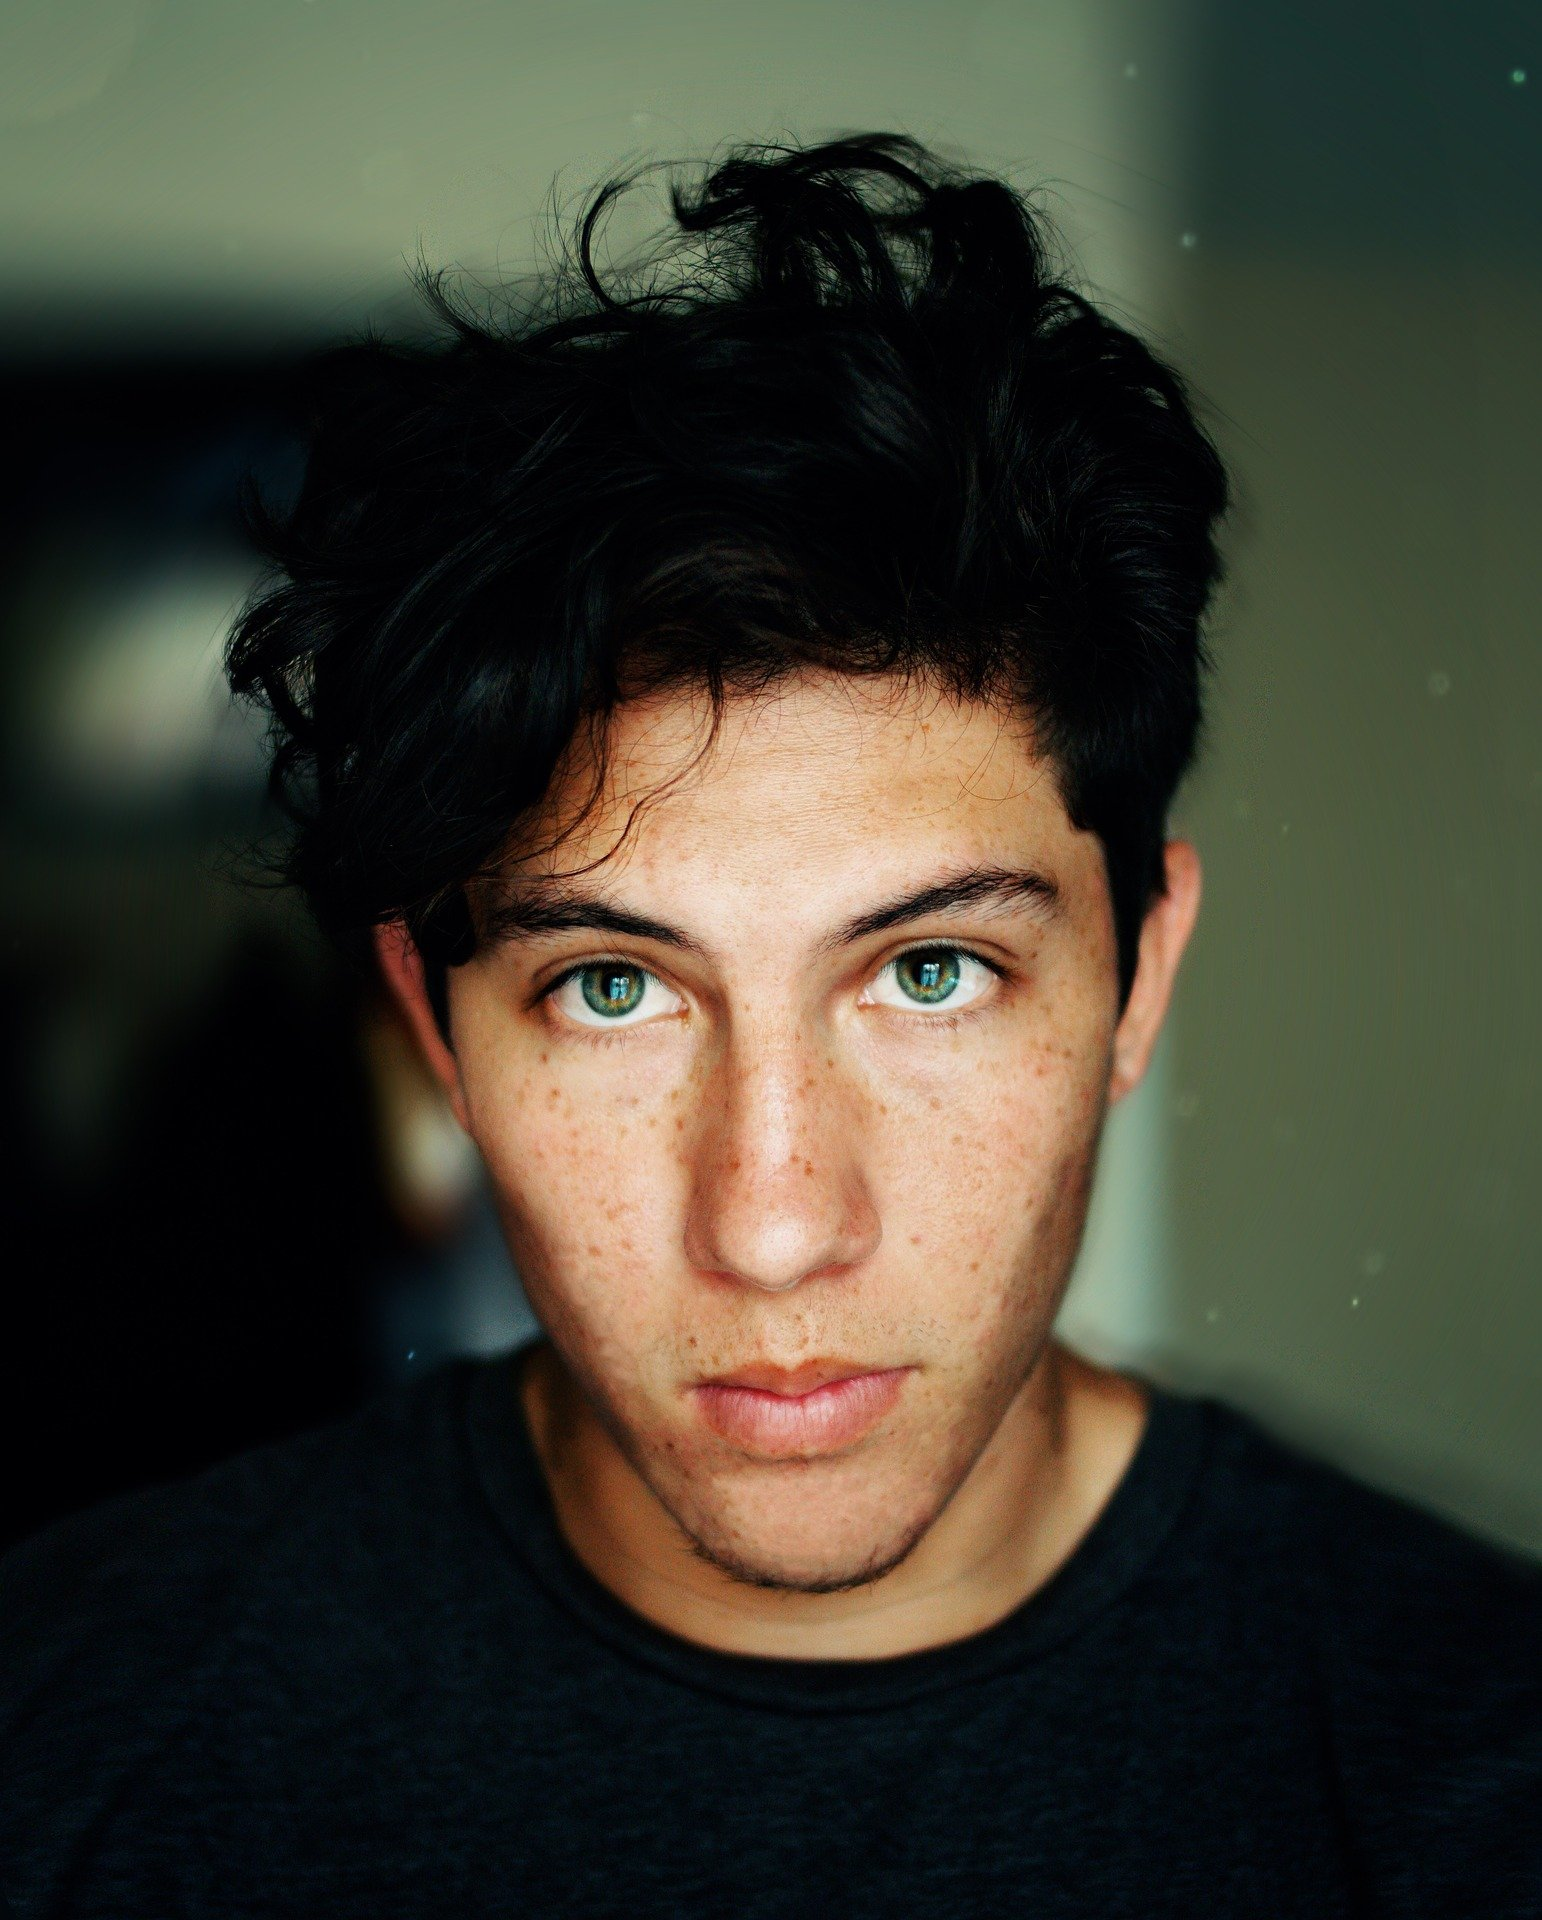
\includegraphics[scale=0.04]{figuras/personas/portrait-3353699_1920.jpg} 
Fonte: Pixabay\tablefootnote{https://pixabay.com/photos/portrait-people-adult-man-face-3353699/}
\end{center} 

&

\textbf{Nome: } Victor Matheus Farias

\textbf{Idade:} 19 anos

\textbf{Ocupação:} Estudante de Engenharia de Software na UnB - Gama.

\\ \hline
\multicolumn{2}{|c|}{\textbf{Descrição Geral}} \\ \hline

\multicolumn{2}{|p{15cm}|}{
    \begin{tabular}[c]{@{}l@{}}\\
    \textbf{Aprender algum conteúdo} é meu o principal objetivo ao usar jogos. Atualmente eu \\\textbf{uso esse tipo de jogo}, mas com uma \textbf{frequência moderada}, não gasto muito tempo\\ com eles. Estou \textbf{começando o curso de IHC} e \textbf{não tenho um conhecimento} \\\textbf{muito técnico} em relação à design de interfaces. O pouco que tenho obtive em \textbf{outras} \\\textbf{disciplinas} da\ faculdade, cursos online e projetos. Quando vou sanar alguma dúvida eu\\ \textbf{pesquiso na internet} e em alguns casos eu pergunto aos \textbf{colegas, o monitor da}\\ \textbf{disciplina ou o professor}.\\ 
    \end{tabular}
}

\\ \hline
\multicolumn{2}{|c|}{\textbf{Aspectos de Qualidade}} \\ \hline

\multicolumn{2}{|p{15cm}|}{
    \begin{tabular}[c]{@{}l@{}}\\
    Um jogo para aprendizagem, deve me ensinar mesmo que eu erre, \textbf{respondendo às}\\ \textbf{minhas ações}, me ensinando; deve ter um \textbf{design legal}; deve ser \textbf{simples de se}\\ \textbf{aprender a jogar}, \textbf{não tendo regras extensas} e tutorias longos. O que mais espero \\de um jogo assim é sentir \textbf{satisfação} em aprender jogando, com uma dose de \textbf{desafios}\\ e \textbf{diversão}. Perceber a \textbf{relevância} do conteúdo é algo que me dá \textbf{confiança} que irei\\ atingir meu objetivo de estudo e mesmo não gastando muito tempo com jogos, se\\ percebesse bons resultados eu me manteria \textbf{focado}.\\
    \end{tabular}
} \\ \hline
\end{tabular}
\legend{Fonte: Autor}
\end{table}
\begin{table}[htbp]
\centering
\caption{Persona Secundária}
\label{tab:Table_persona2}
\small
\begin{tabular}{| m{0.2\textwidth} m{0.7\textwidth}|}
\hline \multicolumn{2}{|c|}{\textbf{Identidade}} \\ \hline
& \\

\begin{center} 
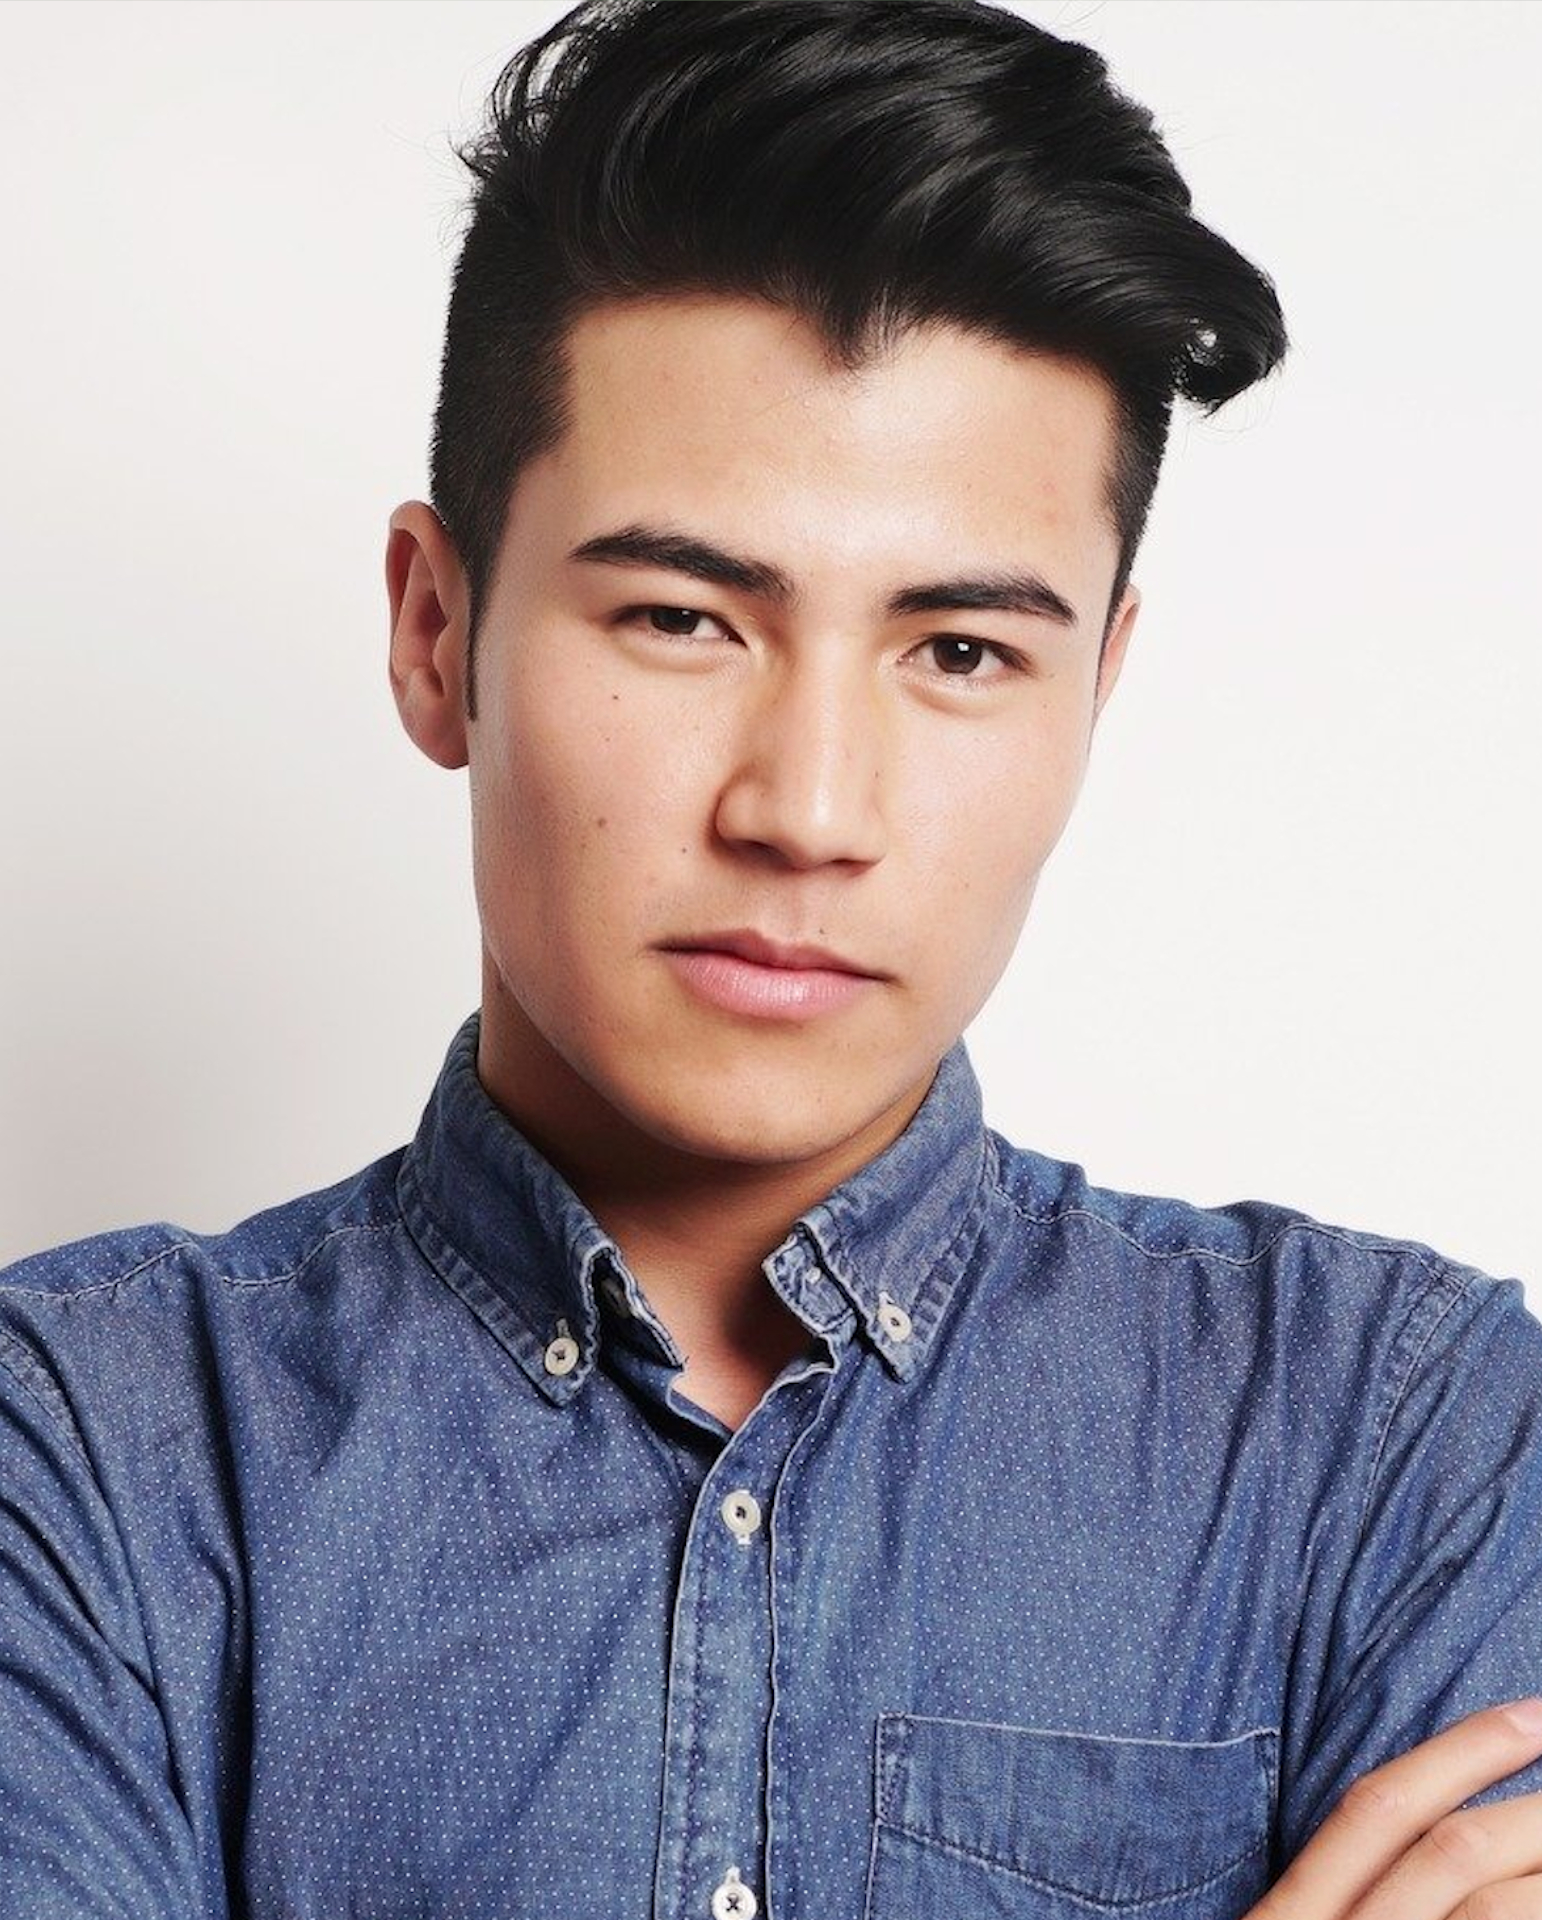
\includegraphics[scale=0.04]{figuras/personas/model-2911332_1920.jpg} 
Fonte: Pixabay\tablefootnote{https://pixabay.com/photos/model-businessman-corporate-2911332/}
\end{center} 

&

\textbf{Nome: } Afonso Souza de Queiroz

\textbf{Idade:} 19 anos

\textbf{Ocupação:} Estudante de Engenharia de Software na UnB - Gama

\\ \hline


\multicolumn{2}{|c|}{\textbf{Descrição}} \\ \hline
\multicolumn{2}{|p{15cm}|}{
     \begin{tabular}[c]{@{}l@{}}\\
        \textbf{Já joguei} alguns jogos para \textbf{aprender um conteúdo} e que me possibilitava \textbf{avaliar} se \\eu realmente tinha aprendido. Eu jogava com certa \textbf{moderação}. Atualmente eu \textbf{não uso} \\\textbf{jogos} desse tipo, mas o motivo é porque eu \textbf{alcancei meus objetivos} de estudo e por\\ enquanto não encontrei nenhum outro jogo que me auxilie. Estou \textbf{cursando IHC}, por\\ isso \textbf{não tenho muito conhecimento} em relação a elaboração de design de interfaces,\\ pois o pouco que tenho veio apenas de projetos de \textbf{outras disciplinas}. Estudo mais \\ sozinho, \textbf{pesquisando na internet} e buscando por conta própria materiais de estudo. \\Apenas quando não encontro, reviso os \textbf{materiais} \textbf{disponibilizados pelo professor} e \\também não descarto a ajuda de \textbf{colegas, monitor} \textbf{da disciplina e do professor}.\\
        \\
        Para mim, um jogo onde vou aprender deve ter um design com um \textbf{padrão simples},\\ mas que desperte \textbf{interesse}; deve me dar bons \textbf{feedbacks} a cada interação que faço;\\ deve ser algo \textbf{simples de aprender a jogar} e \textbf{simples de jogar}, nada muito difícil; e \\seria bom que os \textbf{textos do conteúdo} fossem bem objetivos, com \textbf{cores e fontes} bem\\ ajustadas para a leitura. Espero ter a sensação logo de cara que \textbf{não vou perder meu} \\\textbf{tempo} com o jogo, mas sim que vou \textbf{perceber o quanto o conteúdo é importante} e \\o quanto foi \textbf{satisfatório} ter me \textbf{divertido} aprendendo. E espero também de certa ter \\pequenos \textbf{desafios}, pois isso me ajuda a \textbf{focar} na atividade que estou realizando.\\ \\ 
    \end{tabular}
} \\ \hline
\end{tabular}
\legend{Fonte: Própria Autoria}
\end{table}

\begin{table}[htbp]
\centering
\caption{Persona Suplementar}
\label{tab:Table_persona3}
\small
\begin{tabular}{| m{0.2\textwidth} m{0.7\textwidth}|}
\hline \multicolumn{2}{|c|}{\textbf{Identidade}} \\ \hline
& \\

\begin{center} 
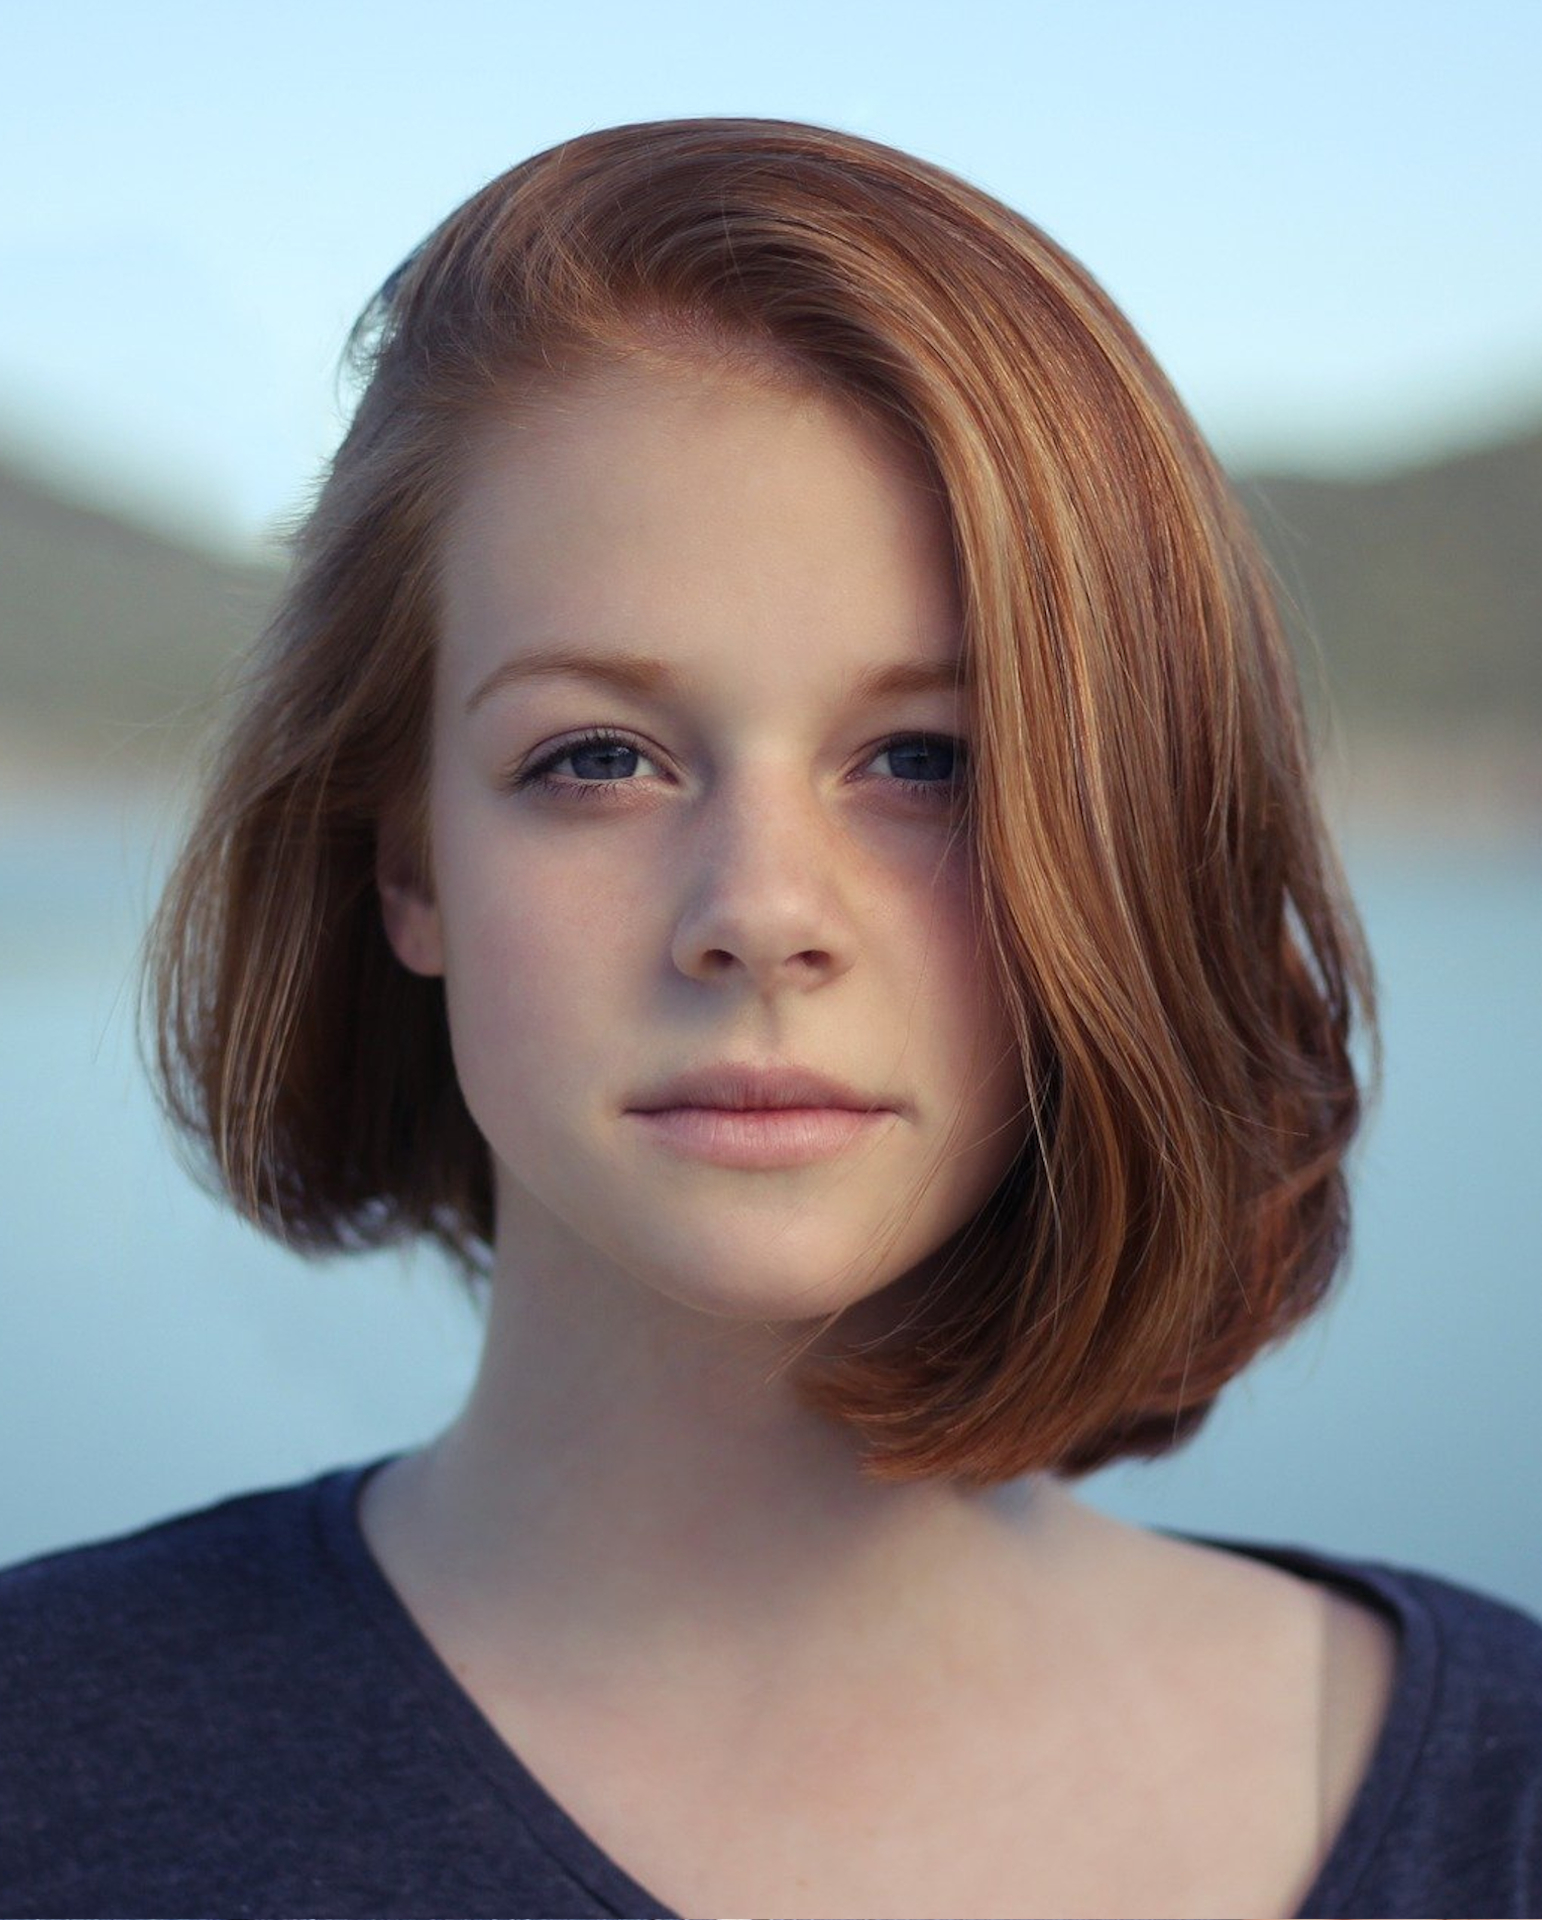
\includegraphics[scale=0.04]{figuras/personas/girl-919048_1920.jpg}
Fonte: Pixabay\tablefootnote{https://pixabay.com/photos/girl-portrait-hairstyle-redhead-919048/}
\end{center} 

&

\textbf{Nome: }  Natália Figueiredo

\textbf{Idade:} 23 anos

\textbf{Ocupação:} Estudante de Engenharia de Software na UnB - Gama.

\\ \hline


\multicolumn{2}{|c|}{\textbf{Descrição}} \\ \hline
\multicolumn{2}{|p{15cm}|}{
    \begin{tabular}[c]{@{}l@{}}\\
        \textbf{Nunca joguei} jogos para aprendizagem, pois \textbf{não conheci nenhum} que tinha o \\propósito de ensinar o que eu desejava. No caso, seria interessante um jogo o qual eu \\pudesse \textbf{aprender} um conteúdo, \textbf{avaliar} o que aprendi e \textbf{revisá-lo} quando necessário.\\ \textbf{Estou no primeiro semestre} da faculdade, por isto \textbf{não tenho conhecimento} em \\relação a elaboração de design de interfaces. Quando vou sanar alguma dúvida que tenho\\ sobre o conteúdo eu \textbf{pesquiso na internet}, \textbf{assisto vídeo aulas}, utilizo do \textbf{material} \\\textbf{disponibilizado pelo professor}. Além de recorrer aos meus \textbf{colegas e quem estiver} \\\textbf{disposto a ajudar}. \\
        \\
        Acho que um jogo para se estudar teria de ter um \textbf{design simples e atraente}, sendo\\ feito um \textbf{bom uso das fontes e core}s, além de uma \textbf{lógica de jogo} e \textbf{regras fáceis} de\\ entender e de se lembrar. Talvez obter \textbf{recompensas} e ter \textbf{feedbacks} evidenciando meu\\ progresso seria interessante. Ao jogar, espero encontrar \textbf{desafios} não muito difíceis, mas\\ que despertem minha \textbf{atenção}. Seria bom, perceber logo de início que o jogo traz um \\\textbf{conteúdo relevante} e que vou \textbf{conseguir aprendê-lo}. E por fim não seria nada ruim\\ sentir \textbf{prazer} em aprender e ainda me \textbf{divertir}.\\
        \\
    \end{tabular}
} \\ \hline
\end{tabular}
\end{table}


\begin{table}[htbp]
\centering
\caption{Anti-Persona}
\label{tab:Table_persona4}
\small
\begin{tabular}{| m{0.2\textwidth} m{0.7\textwidth}|}
\hline \multicolumn{2}{|c|}{\textbf{Identidade}} \\ \hline
& \\

\begin{center} 

\includegraphics[scale=0.04]{figuras/personas/man-1209494_1920.jpg} 
Fonte: Pixabay\tablefootnote{https://pixabay.com/photos/biceps-aesthetics-body-fitness-2746490/}
\end{center} 

&

\textbf{Nome: }  Rafael Medeiros

\textbf{Idade:} 28 anos

\textbf{Ocupação:} Estudante de Educação Física na UnB - Darcy Ribeiro.

\\ \hline


\multicolumn{2}{|c|}{\textbf{Descrição Geral}} \\ \hline
\multicolumn{2}{|p{15cm}|}{
    \begin{tabular}[c]{@{}l@{}}\\
        Não tenho costume de usar jogos para aprendizagem, devo ter jogado uma vez ou outra,\\ mas\textbf{não me interessei muito} e rapidamente \textbf{o jogo se tornou monótono} pra mim e\\ isso me frustrou, pois não alcancei meu objetivo de estudo. Prefiro jogos esportivos como\\ futebol e basquete. Em relação ao conhecimento acadêmico, me concentro apenas nas\\ disciplinas do meu curso. \\
    \end{tabular}
}

\\ \hline
\multicolumn{2}{|c|}{\textbf{Aspectos de Qualidade}} \\ \hline

\multicolumn{2}{|p{15cm}|}{
    \begin{tabular}[c]{@{}l@{}}\\
        No geral, sou bem \textbf{competitivo}, ``dou o sangue'' para \textbf{conquistar} um gol e fazer um \\\textbf{ponto} em qualquer jogo. Em jogos digitais eu gosto de ser envolvido com uma \textbf{história} \\bacana e fico bastante empolgado com gráficos bem realistas e sofisticados. Sou mais fã \\de jogos com \textbf{trabalho em equipe} do que jogos individuais. Gosto tanto atividades \\ lúdicas que se desse pra aprender com elas, com certeza \textbf{trocaria qualquer livro} pra \\aprender me divertindo. \\
        \\
    \end{tabular}
} \\ \hline
\end{tabular}
\legend{Fonte: Autor}
\end{table}

% contar mais um pouco da historinha de como foram definidas as características de cada uma, mostrando o link  da frequencia das respostas com o porque da característica da persona.  


